%

%%%%%%%%%%%%%%%%%%%%%%% file typeinst.tex %%%%%%%%%%%%%%%%%%%%%%%%%
%
% This is the LaTeX source for the instructions to authors using
% the LaTeX document class 'llncs.cls' for contributions to
% the Lecture Notes in Computer Sciences series.
% http://www.springer.com/lncs       Springer Heidelberg 2006/05/04
%
% It may be used as a template for your own input - copy it
% to a new file with a new name and use it as the basis
% for your article.
%
% NB: the document class 'llncs' has its own and detailed documentation, see
	% ftp://ftp.springer.de/data/pubftp/pub/tex/latex/llncs/latex2e/llncsdoc.pdf
%
%%%%%%%%%%%%%%%%%%%%%%%%%%%%%%%%%%%%%%%%%%%%%%%%%%%%%%%%%%%%%%%%%%%


\documentclass[runningheads,a4paper]{llncs}

\usepackage{amssymb}
\usepackage[cmex10]{amsmath}
\setcounter{tocdepth}{3}
\usepackage{graphicx}
\usepackage[noend]{algpseudocode}
\usepackage{algorithm}
%\usepackage{algorithmicx}
\usepackage{url}
\urldef{\mailsa}\path|{carlos.costa, pro09002, jbarbosa}@fe.up.pt|  
\newcommand{\keywords}[1]{\par\addvspace\baselineskip
\noindent\keywordname\enspace\ignorespaces#1}
\algnewcommand{\LineComment}[1]{\State \(\triangleright\) #1}

\begin{document}

\mainmatter  % start of an individual contribution

% first the title is needed
\title{Distributed Prime Sieve in Heterogeneous Computer Clusters}

% a short form should be given in case it is too long for the running head
\titlerunning{Distributed Prime Sieve in Heterogeneous Computer Clusters}

% the name(s) of the author(s) follow(s) next
%
% NB: Chinese authors should write their first names(s) in front of
% their surnames. This ensures that the names appear correctly in
% the running heads and the author index.
%
\author{Carlos M. Costa \and Altino M. Sampaio \and Jorge G. Barbosa}
%
\authorrunning{C. M. Costa, A. M. Sampaio, J. G. Barbosa}
% (feature abused for this document to repeat the title also on left hand pages)

% the affiliations are given next; don't give your e-mail address
% unless you accept that it will be published
\institute{Faculdade de Engenharia da Universidade do Porto\\
Rua Dr. Roberto Frias, s/n 4200-465 Porto, Portugal\\
\mailsa\\
}

%
% NB: a more complex sample for affiliations and the mapping to the
% corresponding authors can be found in the file "llncs.dem"
% (search for the string "\mainmatter" where a contribution starts).
% "llncs.dem" accompanies the document class "llncs.cls".
%

\toctitle{Lecture Notes in Computer Science}
\tocauthor{Authors' Instructions}
\maketitle


\begin{abstract}
Prime numbers play a pivotal role in current encryption algorithms and given the rise of cloud computing, the need for larger primes has never been so high. This increase in available computation power can be used to either try to break the encryption or to strength it by finding larger prime numbers. With this in mind, this paper provides an analysis of different sieve implementations that can be used to generate primes to near $2^{64}$. It starts by analyzing cache friendly sequential sieves with wheel factorization, then expands to multi-core architectures and ends with a cache friendly segmented hybrid implementation of a distributed prime sieve, designed to efficiently use all the available computation resources of heterogeneous computer clusters with variable workload and to scale very well in both the shared and distributed memory versions.

\keywords{sieve of Eratosthenes, wheel factorization, shared memory, distributed memory}
%\keywords{distributed prime sieve, sieve of Eratosthenes, wheel factorization, distributed and parallel computing}
% primality testing algorithms
\end{abstract}


\section{Introduction}
\label{Introduction}

Prime numbers have been a topic of wide research given their important role in securing online transactions using asymmetric public key algorithms such as RSA \cite{standard2012rsa}. In this context prime numbers are used to create the public key that is used by the sender to encrypt the message contents. The reason to use a product of two prime numbers to create the public key is because in the current computer architecture, it is computation infeasible to factor large prime numbers, and thus find the original primes used to create the public key, and used then to decrypt the message (with the progress made in quantum computers, this may not hold for very long). Besides encryption, prime numbers can also be used in hash functions to reduce the risk of collision and in pseudo-random number generators.

Although nowadays is more common to use primality testing algorithms \cite{primality1981lenstra} to find large primes, sieves have been a known method to generate primes up to a given number. One of the most efficient prime number sieve was discovered by Eratosthenes \cite{eratosthenes2009neill} in the ancient Greece and can generate prime numbers up to a given number $n$ with $O(n\log{\log{n}})$ operations. Other prime sieves were discovered since then, such as the sieve of Atkin \cite{atkin2004prime} or the sieve of Sundaram \cite{aiyar1934sundaram}, but a modified sieve of Eratosthenes is still considered to be the most efficient algorithm to use in the current computer architecture, and thus it was the one chosen to be used. 

This paper contributes with an extensive analysis of modified sieve of Eratosthenes algorithm. For that, we have implemented several variants of the algorithm, ranging from sequential form, passing to parallel on multi-core architectures and ending in distributed computer clusters. Each of these 3 main implementations have several algorithm variations, to determine which strategy is more suitable for each usage. As such, it was developed algorithms variations that focus on using the minimum amount of memory, while others focus on computing time, and some make a trade-off between the two. Finally it was implemented several segmented versions of both parallel and distributed algorithms to allow the computation of primes to near the maximum number represented by the current computer architecture ($2^{64}$). Special attention was devoted to the distributed algorithms since they provide the most suitable implementation that can be used to calculate primes near $2^{64}$ in reasonable time. The restriction to limit the range to near $2^{64}$ aims to avoid overflow of numbers when sieving. To achieve this, the maximum limit is lowered to $2^{64} - 2 \sqrt{2^{64}} - 1$. This guarantees that the maximum number that can be used as a seed will not cause overflow. This version is designed to scale well to large clusters and is implemented to perform dynamic allocation of segments to nodes in order to efficiently use all the computation resources of clusters with heterogeneous hardware and with variable workload. The implemented algorithms are assessed in terms of speedup, efficiency and scalability.

The remainder of this paper is organized as follows. Section II discusses related work. Section III first introduces some background information that are the starting point of the proposed algorithms, and then the several implementation versions are described. Section IV analyzes the results obtained and Section VI concludes the paper.


\section{Related Work}
\label{Related Work}

The generation of prime numbers have been a topic of wide research essentially due to their need for the creation of key pairs or as a computation stage during various cryptographic setups. Singleton et al. \cite{singleton1969efficient} published in 1969 the first segmented version of the sieve of Eratosthenes. Based in the sieve of Eratosthenes, Shahid et al. \cite{bokhari1987multi} implemented a parallel version on the Flex/32 shared memory multiprocessor at NASA Langley Research Center. The author have studied the impact of several parameters in its performance, and concluded that there is no advantage in using more than four or five processors unless dynamic load balancing is employed. Anderson et al. \cite{anderson1988ada} implemented an Ada program which uses a multitasking solution for the Sieve of Eratosthenes. Authors illustrate the power and flexibility of Ada in achieving concurrent solutions, and the capacity of the program to be used as a benchmark program for evaluating multiple CPU systems. Shapiro et al. \cite{shapiro1989family} described a modification to the Sieve of Eratosthenes implementing a concurrent solution algorithm for multi-processor computers. Sorenson et al. \cite{sorenson1994fast} have presented two parallel prime number sieves. They proposed two algorithms and show that the first sieve runs in $O(\log{n})$ time using $O(n/(\log{n} \log{\log{n}}))$ processors, while the second sieve runs in $O(\sqrt{n})$ time using $O(\sqrt{n})$ processors. Authors clarify that the second algorithm is more efficient when communication latency is high. 

From all the publicly implementations analyzed, special interest was devoted to the Prime Sieve \cite{kim2013} developed by Kim Walisch, which is considered to be the fastest multi-core implementation publicly available at the present date. Other papers that influenced the strategies developed included \cite{jarai2011cache} that details a very efficient use of the cache memory system for very large prime numbers. Additionally, \cite{paillard2005fully} \cite{sorenson1991analysis} explain how to use wheel factorization to considerably speed up the sieving process, and \cite{david2009parallel} \cite{cordeiro2012parallelization} provide insights on how to implement the simple MPI \cite{gropp1999mpi} version. However, as far as we know, there is no available implementation that can compute prime numbers in a distributed memory architecture, in order to allow the computation of prime numbers up to $2^{64}$ in reasonable time.


\section{Background}
\label{Background}

In this section we present a brief explanation of the main concepts used in our proposals.

\subsection{Sieve of Eratosthenes}
\label{Sieve of Eratosthenes}

The sieve of Eratosthenes \cite{eratosthenes2009neill} was invented in ancient Greece by Eratosthenes around the $3^{rd}$ century B.C., and describes a method for calculating primes up to a given number $n$ in $O(n \log{\log{n}})$ operations. The Algorithm \ref{alg:sieve_eratosthenes} describes the pseudo code of the sieve of Eratosthenes:


\begin{algorithm}[h]
        \begin{algorithmic}[1]
                \State \textbf{Input:} an integer $n > 1$
                \LineComment{Let P be an array of Boolean values, indexed by integers 2 to n, initially all set to true}
                \Statex
                \For{$i \in \{2, 3, 4, ..., n$\}}
                        \If {$P[i] == true$} 
                                \For{$j \in \{2i, 3i, 4i, ..., n$\}}
                                        \State $P[j] = false$
                                \EndFor
                        \EndIf
                \EndFor
                \Statex
                \LineComment{Now all i, such that P[i] is true, are prime numbers}
        \end{algorithmic}
        \caption{Sieve of Eratosthenes}
        \label{alg:sieve_eratosthenes}
\end{algorithm}

This algorithm finds all the prime numbers less than or equal to a given integer $n$. For that, it creates a list of integers from 2 to $n$ (line 3), and then, starting in 2, the first prime number, it marks all items in the list that are integers multiple of 2 (line 6). It then repeats the process for the next item in the list that is not marked (which is the next prime), until there is no such item. 


\subsection{Wheel Factorization}
\label{Wheel Factorization}

Wheel factorization \cite{pritchard1982wheel} is a known optimization used to cross off multiples of several sieving primes. It can be used to considerable speed up the sieving process if used efficiently.

A modulo 30 wheel, which has sieving primes 2, 3 and 5, can cross off as much as 66\% of composites. 
A modulo 210 wheel, which besides sieving primes 2, 3 and 5 also has prime 7, can increase the percentage of removed composites to 77\%.
Larger wheels may not have a reasonable improvement in \% of composites crossed off, because the table required for the wheel factorization [14] may not fit in the cache memory. The creation of the wheel sieve table is described by Algorithm \ref{alg:wheel_factorization}:

\begin{algorithm}[h]
        \begin{algorithmic}[1]
                \State \textbf{Input:} a P list of known prime numbers
                \LineComment{Let m be the product of the known prime numbers in the P list}
                \LineComment{Let C be an array of Boolean values with numbers in [1, m], initially all set to false}
                \Statex
                \For{$i \in P$}
                        \For{$j \in \{2i, 3i, 4i, ..., m$\}}
                                \State $C[j] = true$
                        \EndFor
                \EndFor
                \Statex
                \LineComment{Now for all x numbers such as k=(x modulus m) in [1, m], if C[k] is false, then x is a probable prime number, and needs to be checked by other means to confirm if it is a prime number or not. If C[k] is true, then x is a composite number of one of the primes in list P}
        \end{algorithmic}
        \caption{Wheel Factorization}
        \label{alg:wheel_factorization}
\end{algorithm}


The purpose of wheel factorization is to skip multiples of small primes. In this regarding, if the $k^{th}$ wheel is added to the sieve of Eratosthenes, then any multiples that are divisible by any of the first k primes are skipped. For example, the $1^{st}$ wheel considers only odd numbers, the $2^{nd}$ wheel (modulo 6) skips multiples of 2 and 3, the $3^{rd}$ wheel (modulo 30) skips multiples of 2, 3, 5 and so on \cite{kim2013}.

By applying the wheel factorization method, the running time of the sieve of Eratosthenes can be reduced by a factor of $\log{\log{n}}$ if the wheel size is $\sqrt{n}$ \cite{pritchard1983fast}.


\section{Proposed Solutions}
\label{Proposed Solution}

In the following sections we present the main concepts behind each prime sieve algorithm implemented. The order used denotes the development of each variation in relation to the previous ones and aims to facilitate the identification of the optimizations that were introduced in each development iteration.

In the simple algorithms the pseudo code is provided to facilitate the explanation of the algorithm. However, given the length of the algorithms, for the more optimized versions, it is only explained the main concepts. The implementation source code is available in \cite{costa2013}.

\subsubsection{Sequential Prime Sieve Using Trial Division (v.1):}
\label{Sequential Prime Sieve Using Trial Division}

Algorithm \ref{alg:alg_1} is one of the simplest methods to compute prime numbers. It works by crossing off all odd $j$ numbers that are composite of a previous prime number $i$. This can be achieved by checking if a $j$ number is multiple of a previous prime number ($i$) by using the modulus operator. If the remainder of the integer division between $j$ and $i$ is 0, then $j$ is multiple of $i$ and is marked as composite.

One optimization applied that improves upon the original Eratosthenes algorithm is that the sieving can start at $i^2$ instead of $2i$ in order to avoid marking a composite number multiple times. For example 21 is multiple of 3 and 7, so there is no need to mark it as composite when sieving with prime 7 because it was already sieved with the prime 3. For the same reason, it is only necessary to check $i$ until $\sqrt{n}$, because when $i > \sqrt{n}$, the $j$ will exceed $n$ and as a result, the code in line 7 will never be executed.

Another optimization is to completely exclude even numbers, and this way reduce the computations and memory to half. This will require an adjustment in the way the numbers are mapped to memory positions ($[j - 3 / 2]$ instead of $[j]$) and will increase the increment necessary to transition to the next number ($+2$ instead of $+1$ in line 5).

\begin{algorithm}[h]
        \begin{algorithmic}[1]
                \State \textbf{Input:} an integer $n > 1$
                \LineComment{Let C be an array of Boolean values representing the odd numbers $> 1$, initially all set to false}
                \Statex
                \For{i $\in \{3, 5, 7, ..., \sqrt{n}$\}}
                        \If {$C[(i - 3) / 2] == false$} 
                                \For{$j \in \{i^2, i^2 + 2, i^2 + 4, ..., n$\}}
                                        \If {$j \; \% \; i == 0$}
                                                \State $C[(j - 3) / 2] = true$
                                        \EndIf
                                \EndFor
                        \EndIf
                \EndFor
                \Statex
                \LineComment{Now all the positions in array C still marked as false, represent prime numbers}
        \end{algorithmic}
        \caption{Sequential Prime Sieve Using Trial Division (v.1)}
        \label{alg:alg_1}
\end{algorithm}


\subsubsection{Sequential Prime Sieve Using Fast Marking (v.2):}
\label{Sequential Prime Sieve Using Fast Marking}

Algorithm \ref{alg:alg_1} is very inefficient because it uses modulus operations to check for composites, which is a very computational intensive task, especially if the maximum range to sieve is a large number.

An alternative is to use additions instead of modulus operations, because they are much faster to compute. The  idea is to cross off all $j$ numbers that we already know that are composites, because $i^2 + k \times i$ is guaranteed to be a composite of number $i$.

As shown in Algorithm \ref{alg:alg_2}, another optimization is that the increment to mark the next composite can be $2i$ since adding $i$ to an odd multiple of $i$ will result in an even number (even numbers are not prime).

\begin{algorithm}[h]
        \begin{algorithmic}[1]
                \State \textbf{Input:} an integer $n > 1$
                \LineComment{Let C be an array of Boolean values representing the odd numbers $> 1$, initially all set to false}
                \Statex
                \For{i $\in \{3, 5, 7, ..., \sqrt{n}$\}}
                        \If {$C[(i - 3) / 2] == false$} 
                                \For{$j \in \{i^2, i^2 + 2i, i^2 + 4i, ..., n$\}}
                                        \State $C[(j - 3) / 2] = true$
                                \EndFor
                        \EndIf
                \EndFor
                \Statex
                \LineComment{Now all the positions in array C still marked as false, represent prime numbers}
        \end{algorithmic}
        \caption{Sequential Prime Sieve Using Fast Marking (v.2)}
        \label{alg:alg_2}
\end{algorithm}


\subsubsection{Sequential Prime Sieve Using Fast Marking With Block Decomposition Optimized For Space (v.3):}
\label{Sequential Prime Sieve Using Fast Marking With Block Decomposition Optimized For Space}

Although Algorithm \ref{alg:alg_2} is considerable faster than Algorithm \ref{alg:alg_1}, it suffers from performance degradation by not using the cache memory system efficiently. This happens because the same areas of array $C$ are being loaded to cache memory more times than necessary, since the algorithm is sieving the composites of each prime number $i$ to the end of array $C$. This is extremely inefficiently, because each cache miss forces the CPU to wait hundreds of clock cycles to load data from the main memory.

To solve this problem, Algorithm \ref{alg:alg_3} implements a sieve with block decomposition (splits the sieving range in blocks that fit in the cache), in order to load the values of the array $C$ only one time (to the cache), and then sieve all primes numbers up to $\sqrt{n}$ in that block, before moving to the next.

\begin{algorithm}[h]
        \begin{algorithmic}[1]
                \State \textbf{Input:} an integer $n > 1$
                \LineComment{Let C be an array of Boolean values representing the odd numbers $>$ 1, initially all set to false}
                \LineComment{Let bs be the block size in number of elements}
                \LineComment{Let nb = n / bs be the number of blocks to use in sieving}

                \Statex
                \State \Call{calculatePrimesInBlock}{3, 3 + bs} \Comment{First block}
                
                \For{b $\in \{1, 2, 3, ..., nb$\}} \Comment{Remaining blocks}
                        \State $a = b \times bs$
                        \State $b = a + bs$     \Comment{Last block should have an upper limit of n + 1, because they are sieved in range [a, b[}

                        \State \Call{removePrimesFromPreviousBlocks}{a, b}
                        \State \Call{calculatePrimesInBlock}{a, b}
                \EndFor
                \LineComment{Now all the positions in array C still marked as false, represent prime numbers}
				\Statex
                \Function{calculatePrimesInBlock}{$a, b$} \Comment{Sieves in range [a, b[}
                        \For{i $\in \{a, a+2, a+4, ..., \sqrt{n}\}$}
                                \If {$C[i] == false$}
                                        \For{j $\in \{i^2, i^2+2i, i^2+4i, i^2+6i, ..., b$\} } \Comment{Not including b}
                                                \State $C[j] = true$
                                        \EndFor
                                \EndIf
                        \EndFor
                \EndFunction

				\Statex
                \Function{removePrimesFromPreviousBlocks}{$a, b$} \Comment{Sieves in range [a, b[}
                        \For{i $\in \{0, 1, 2, ..., k$\} } \Comment{k not exceeding the position in C associated with $\sqrt{n}$}
                                \If {$C[i] == false$}
                                        \State p = closest prime multiple of number associated with position i in relation to a
                                \EndIf

                                \For{j $\in \{p, p + 2p, p + 4p, ..., b$\} } \Comment{Not including b}
                                        \State $C[j] = true$
                                \EndFor
                        \EndFor
                \EndFunction
        \end{algorithmic}
        \caption{Sequential Prime Sieve Using Fast Marking With Block Decomposition Optimized For Space (v.3)}
        \label{alg:alg_3}
\end{algorithm}


\subsubsection{Sequential Prime Sieve Using Fast Marking With Block Decomposition Optimized For Time (v.4):}
\label{Sequential Prime Sieve Using Fast Marking With Block Decomposition Optimized For Time}

Algorithm \ref{alg:alg_3} has a section of code (line 20) that is constantly repeating computations. That section is the calculation of the closest prime number in relation to the beginning of the block. In order to prevent this repetition, this version keeps in memory the last prime multiple associated with each prime (that was computed in the previous block). And since it is only necessary to store the prime multiples associated to primes up to $\sqrt{n}$, this represents a very reasonable trade-off between space and computation time. 

This is the first variation in which a segmented sieve was implemented, in order to try to save some memory by keeping the bitset of booleans only for the current block. But since all the primes found are kept in memory instead of being compacted in the bitset, it ends up consuming much more memory because each prime has 64 bits of storage.


\subsubsection{Sequential Prime Sieve Using Fast Marking With Block Decomposition Optimized For Space and Time (v.5):}
\label{Sequential Prime Sieve Using Fast Marking With Block Decomposition Optimized For Space and Time}

This variation is implemented to reduce even more the repetition of computation that occur in the previous algorithm and to revert to the previous memory scheme.

The improvement is to avoid the repetition of the computation of the double of a prime to use as an increment in the \mbox{\textit{removePrimesFromPreviousBlocks}} function in Algorithm \ref{alg:alg_3} (line 21). As such, once the prime double is calculated for the first time in \mbox{\textit{calculatePrimesInBlock}} function in the same algorithm, it is associated to the prime multiple. Since there are very few primes to sieve in comparison to the maximum range of sieving, saving a pair of the current prime multiple and its double to avoid constant repetition of computations is very reasonable.


\subsubsection{Sequential Prime Sieve Using Fast Marking With Block Decomposition Optimized For Space With Modulo 30 or 210 Wheel Factorization (v.6 and v.7):}
\label{Sequential Prime Sieve Using Fast Marking With Block Decomposition Optimized For Space With Modulo 30 or 210 Wheel Factorization}

This alternative introduces the wheel factorization to speed up the sieving process. Instead of using the wheel factorization to pre-sieve numbers and update the bitset of composite numbers, this implementation uses the wheel sieve to determine the next possible prime given a number. This way the bitset is only updated in the positions that represent possible primes. This variation of use of the wheel sieve is more efficient for sieving, but also implies that to extract the primes from bitset only the positions associated with possible primes must be evaluated, since the others are not considered in the sieving process. With this insight, the access to the bitset is changed in order to store only bits associated with possible primes, and the memory consumption is reduced.

A version with a 30 wheel and 210 wheel was implemented to see the impact of different wheel sizes.


\subsubsection{Sequential Prime Sieve Using Fast Marking With Block Decomposition Optimized For Space and Time and With Modulo 30 or 210 Wheel Factorization (v.8 and v.9):}
\label{Sequential Prime Sieve Using Fast Marking With Block Decomposition Optimized For Space and Time and With Modulo 30 Wheel Factorization}

Since the use of the wheel to store only bits of possible primes introduces a lot of overhead (in the computation of the index to store the result in the bitset), this version reverts to the previous scheme of storing all odd numbers, and uses the wheel to skip the sieving of the composites of the prime numbers 2, 3 and 5 (and also the number 7 in the 210 wheel version). This way, it is expect to obtain a significant performance boost in comparison with the algorithms that did not use wheels and to mitigate the overhead associated with the computation of the bitset indexes when storing only numbers in the wheel.


\subsubsection{Sequential Prime Sieve Using Fast Marking With Block Decomposition Optimized for Time and With Modulo 30 or 210 Wheel Factorization (v.10 and v.11):}
\label{Sequential Prime Sieve Using Fast Marking With Block Decomposition Optimized for Time and With Modulo 30 Wheel Factorization}

Since memory access is a bottleneck in all sieving algorithms, these versions try to determine if using direct memory access without any need to offset calculations would improve performance. The only difference between these variations and the previous ones is that it reserves memory for all numbers, so that the number itself is the position within the bitset where the sieve analysis is going to be stored.


\subsubsection{Parallel Prime Sieve Using Fast Marking With Block Decomposition Optimized for Space or Time and With Modulo 210 Wheel Factorization (v.12 and v.13):}
\label{Parallel Prime Sieve Using Fast Marking With Block Decomposition Optimized for Space and Time and With Modulo 210 Wheel Factorization}

With current computer architectures, any computer intensive algorithm should be designed to take full advantage of the parallel computation resources available in multicore systems. Given that the previous algorithms are already implemented using block decomposition, and that the multicore systems use shared memory, porting the best sequential algorithm (v.9) to a parallel architecture using OpenMP \cite{dagum1998openmp} only requires minor changes to the source code. This approach results in assigning groups of blocks to different threads, and optimizing the allocation of these blocks in order to avoid load unbalancing between the different threads.
Implementation 13 is a port of the version 11 to a parallel architecture.


\subsubsection{Segmented Parallel Prime Sieve Using Fast Marking With Block Decomposition Optimized for Space and Time and With Modulo 210 Wheel Factorization (v.14):}
\label{Segmented Parallel Prime Sieve Using Fast Marking With Block Decomposition Optimized for Space and Time and With Modulo 210 Wheel Factorization}

Since the parallel algorithms were very fast to sieve primes up to $2^{32}$ (about a second), it was developed a segmented variant to allow the computation of primes to near $2^{64}$ using only the amount of memory that is specified in the command line arguments. This way, the algorithm can adapt to different hardware and still compute all primes requested with very little overhead (about 3\%) compared with the fastest OpenMP version (v.13). This overhead is associated with the management of the segments (groups of blocks) and reseting the bitset values (when moving to a new segment).


\subsubsection{Distributed Prime Sieve Using Fast Marking With Block Decomposition Optimized for Space and Time and With Modulo 210 Wheel Factorization (v.15):}
\label{Distributed Prime Sieve Using Fast Marking With Block Decomposition Optimized for Space and Time and With Modulo 210 Wheel Factorization}

This is the first implementation of a distributed prime sieve algorithm prepared to run in homogeneous computer clusters.
It uses the best sequential algorithm (v.9), and splits evenly the workload among the processes (that can be in different computers).
In order to keep communication between processes to a minimum, each process computes the primes up to $\sqrt{n}$ and then uses them to sieve their share of the workload.
The share of the workload [startNumber, endNumber[ is computed as presented in equation \ref{eq:alg_15}:

\begin{equation}
        \begin{split}
                startNumber = \frac{processID \times maxRange}{numberProcessesInWorkgroup}       \\
                endNumber = \frac{(processID + 1) \times maxRange}{numberProcessesInWorkgroup}, \\      processID \in [0, numberProcessesInWorkgroup - 1]
        \end{split}
        \label{eq:alg_15}
\end{equation}


\subsubsection{Distributed Prime Sieve Using Fast Marking With Block Decomposition Optimized for Time and With Modulo 210 Wheel Factorization (v.16):}
\label{Distributed Prime Sieve Using Fast Marking With Block Decomposition Optimized for Time and With Modulo 210 Wheel Factorization}

This is the same algorithm as above but using one less operation (shift left 1 for dividing the number by 2) per memory access. Is similar to previous algorithms optimized for time, but since the algorithm is now segmented, direct memory access can't be done.


\subsubsection{Hybrid Distributed Prime Sieve Using Fast Marking With Block Decomposition Optimized for Space and / or Time and With Modulo 210 Wheel Factorization (v.17 and v.18):}
\label{Hybrid Distributed Prime Sieve Using Fast Marking With Block Decomposition Optimized for Space and / or Time and With Modulo 210 Wheel Factorization}

The previous implementation completely disregards the fact that each node in the workgroup may be a multicore system, and as such, a hybrid version would take better advantage of the shared memory architecture to avoid the replication of the computation of the sieving primes up to $\sqrt{n}$ in the same node. This way, OpenMPI can be used to coordinate the distribution of the workload between different nodes in the cluster and then inside each node can be used an OpenMP variant optimized to take full advantage of the shared memory architecture.

Implementation 18 is a modification of version 17 to use one less operation per memory access (similar to the memory access method introduced in version 16).


\subsubsection{Hybrid Distributed Prime Sieve Using Fast Marking With Block Decomposition Optimized for Space and / or Time, With Modulo 210 Wheel Factorization and With Dynamic Scheduling (v.19 and v.20):}
\label{Hybrid Distributed Prime Sieve Using Fast Marking With Block Decomposition Optimized for Space and Time, With Modulo 210 Wheel Factorization and With Dynamic Scheduling}

The previous distributed hybrid algorithms didn't take into account that the cluster in which they may be used can have heterogeneous hardware nodes with different processing capabilities, and even if the cluster is homogeneous, it may very well have variable workload. These external factors may have a damaging effect on the performance of the previous algorithms because some nodes may finish much sooner than others and then became idle, while others are still processing at full load. In order to avoid this, it was implemented a dynamic scheduling algorithm based in the implementation 18, but with a control process that creates a given number of segments (specified by the user), and then distributes these segments dynamically according to the requests of the nodes that finish their segments. This way, if there is any node that finishes sooner than others, it can continue contributing to the computation by requesting a new segment from the control process. With this strategy, the algorithm is ready to adapt to heterogeneous clusters with variable workloads and can be fine-tuned to a given network topology by specifying how many segments should be created, how many processes should be started and in which nodes, and how many threads should each process use.

Implementation 20 is a modification of version 19 to use one less operation per memory access (similar to the memory access method introduced in version 16).


\section{Results and Discussion}
\label{Results and Discussion}

This section presents the obtained results and the analysis of the algorithms according to different performance metrics. Detailed explanation of the reasons behind the different performances in each algorithm is presented in Section \ref{Performance Analysis}.

These results were collected using Ubuntu 13.04 64 bits, and the source code (available in \cite{costa2013}) was compiled with -O3 -s flags using mpic++ with g++ 4.7.3 and OpenMPI 1.4.5.

The sequential and parallel versions were tested on a laptop (Clevo P370EM) with an Intel i7-3630QM (quad core processor with Hyper-Threading - 2400 MHz clock rate) and 16 GB of RAM DDR3 1600 MHz.

For the distributed algorithms, it was added a second laptop (Asus G51J) with an Intel i7-720QM (quad core processor with Hyper-Threading - 1600 MHz clock rate) and 4 GB of RAM DDR3 1066 MHz. The router for connecting the two laptops was a Technicolor TG582n with 100 Mbps Ethernet connection.


\subsection{Global Performance Analysis}
\label{Global Performance Analysis}

In Figure \ref{fig:global_perf_comparison} is given a global overview of the performance of some of the implementations in ranges from $2^{25}$ to $2^{32}$. The chart shows that most algorithms need a range of about $2^{28}$ to reach their maximum performance. The only exceptions are the distributed algorithms, because the computation capacity was increased roughly 50\% by adding a second node to the workgroup. As such, the performance reaches its maximum in ranges larger than $2^{32}$. The reason for this is related to network latency and initializations overhead of processes and threads taking a considerable percentage of total computation time when the useful computations are relatively small (less than a second).

\begin{figure}[h]
        \centering
        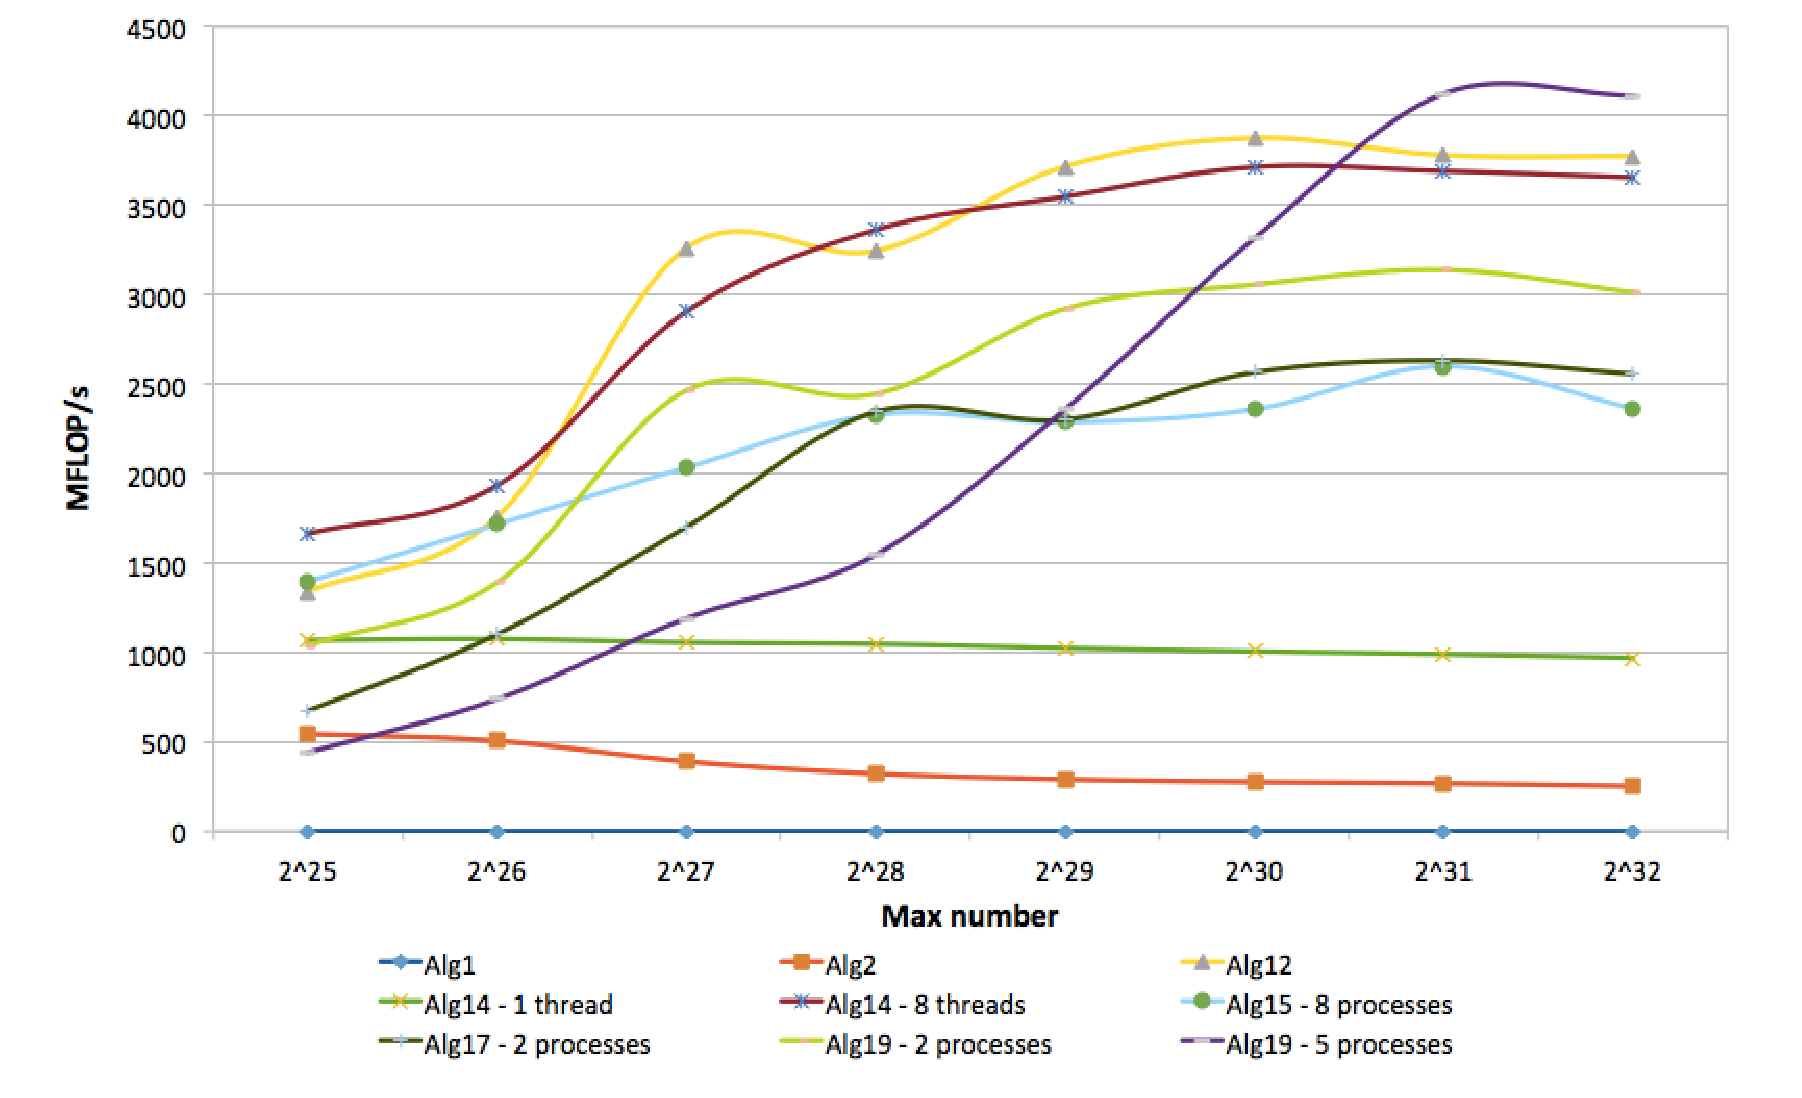
\includegraphics[height=7.0cm]{images/global_perf_comparison}
        \caption{Global performance comparison (Mflops).}
        \label{fig:global_perf_comparison}
\end{figure}

Additionally, we notice that the sequential prime sieves using 30 or 210 wheel factorization achieved a significant performance boost in comparison with the algorithms that did not use wheels.

Since memory access has a significant impact on the runtime of the sieving algorithms, several access and store methods were tested. The fastest way to access a memory position is using the number itself as an index. But results shown that although this is true for small ranges, that doesn't hold for larger ranges (bigger than $2^{25}$). The possible reason may be related to the fact that with this strategy, only half of the numbers can be stored in cache (comparing to implementations that only store even numbers). And as such, although the overhead to access memory is reduced (by not having to calculate the associated index to a given number), the net loss in cache misses starts to outweigh the improved memory access when the range is increased.

Moreover, given the results, implementation 14 is the recommend algorithm to use in single node multicore systems, when it is required to calculate very large primes (bigger than $2^{35}$), using efficiently the memory available, because it is a segmented sieve optimized for good cache usage.

For very large ranges (bigger than $2^{48}$), implementation 19 is the appropriate algorithm to use in a multi node, multi core system, since is can dynamically distribute the computation across several nodes with varying number of cores, by employing a dynamic scheduling / load balancing architecture.


\subsection{Performance Analysis}
\label{Performance Analysis}

In this subsection we analyze the obtained results according to different metrics.

\subsubsection{Real Speedup Metric:}
\label{Real Speedup Metric:}

Figure \ref{fig:real_speed_up} shows the obtained speedup when comparing execution times of the recommended parallel implementation v.14 and distributed implementation v.19, with the best sequential implementation v.9.

\begin{figure}[h]
        \centering
        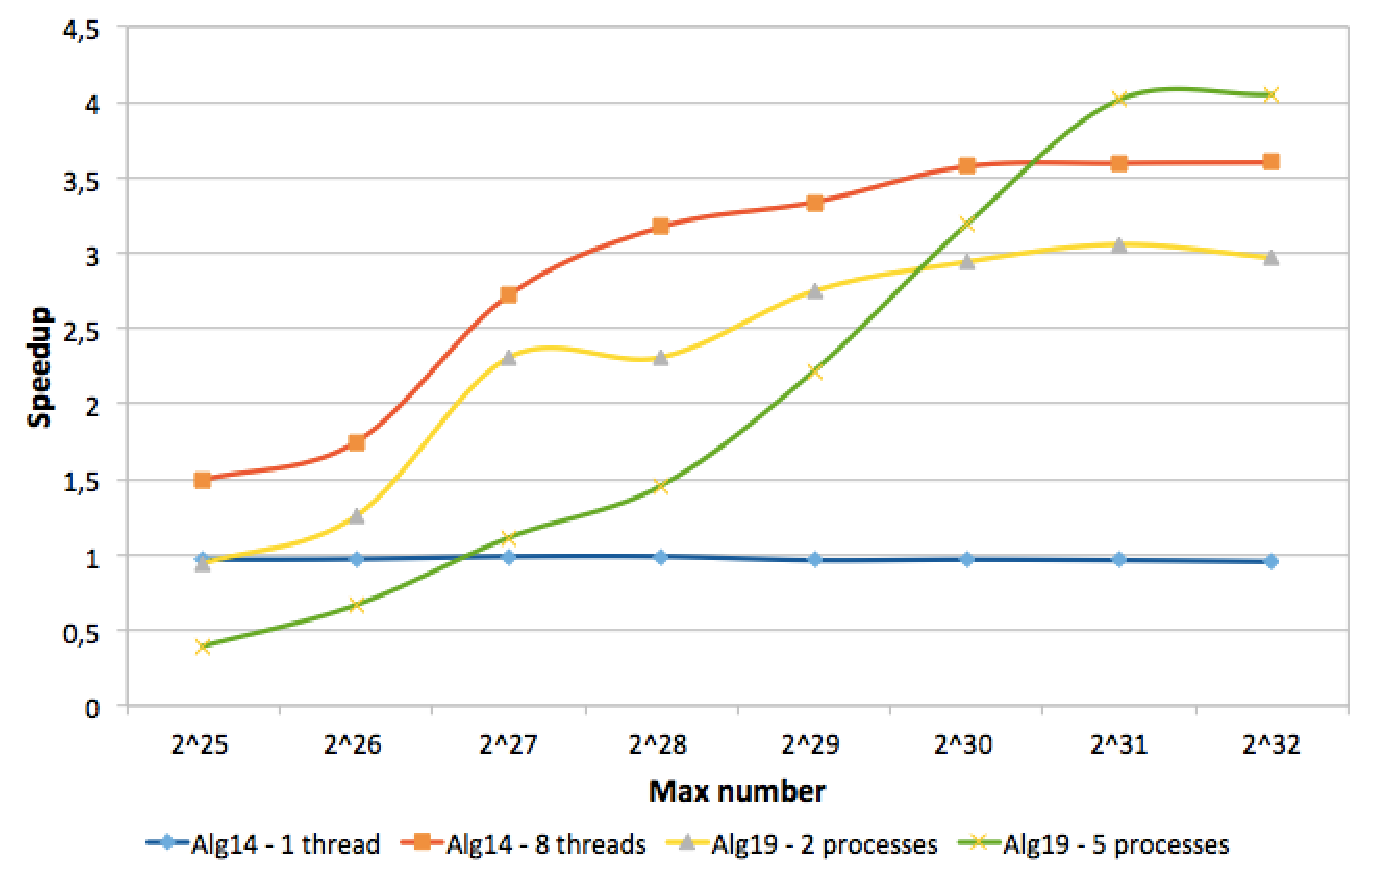
\includegraphics[height=7.0cm]{images/real_speed_up}
        \caption{Real speedup due to different strategies implemented.}
        \label{fig:real_speed_up}
\end{figure}

The results show that the parallel version in implementation v.14 runs best when using 8 threads on a quad core system with hyper-threading. But as expected, the result is not proportional to the number of threads but proportional to the number of real available cores. The speedup is not 4 because there is some sequential sections in the algorithm that cannot be parallelized. It is also clear that the distributed algorithm should only be used for large ranges, since the overhead and latency of MPI calls can damage performance if the total computations are small. The speedup of the distributed version isn't higher because the second node has 50\% less processing capability and uses a 50\% slower memory when compared with the first node. This was done on purpose to determine the adaptability of the algorithm to heterogeneous nodes.


\subsubsection{Efficiency:}
\label{Efficiency:}

Figure \ref{fig:efficiency} shows the obtained efficiency when comparing execution times of the recommended parallel implementation v.14 and distributed implementation v.19, with the best sequential implementation v.9. It was calculated based on the real speedup presented earlier.

\begin{figure}[h]
        \centering
        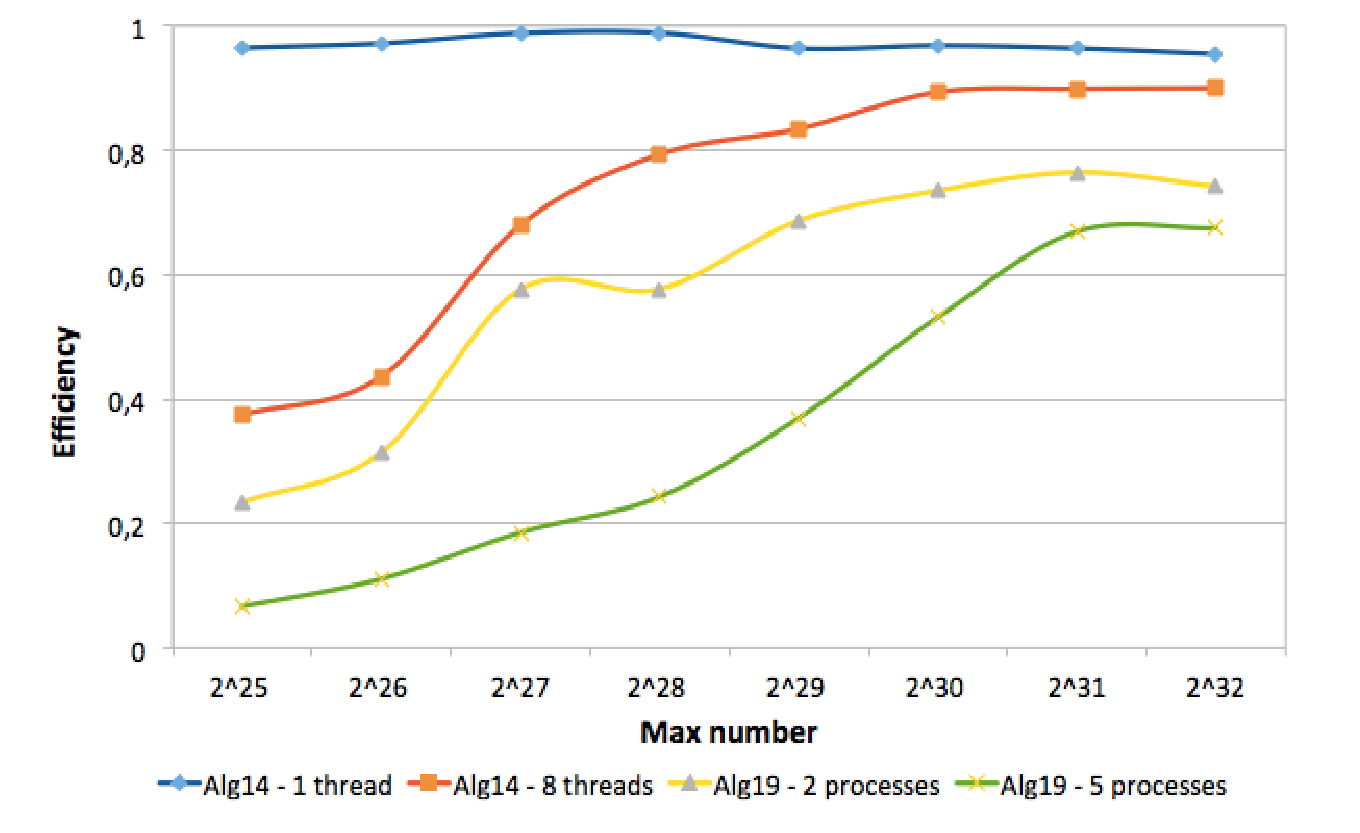
\includegraphics[height=7.0cm]{images/efficiency}
        \caption{Efficiency for two versions of the parallel algorithm}
        \label{fig:efficiency}
\end{figure}

As expected, the best efficiency was obtained with the shared memory algorithm, since it keeps computation repetitions to a minimum (the distributed implementations need to calculate the sieving primes in each process) and doesn't suffer from overhead of MPI calls and latency associated with network communications. The reason for having 5 processes in implementation v.19 when running in 2 nodes is related to the fact that 1 process is only to control the dynamic allocation of segments to the other 4 slave processes, and because on the current testing system, using only one process per node was resulting in lower performance, due to latency in the MPI calls when requesting a new segment from the control process. As such, the performance improves with 2 processes per node, because this way, when 1 process is waiting for a new segment allocation, the other one can still be using the node computation resources. With this strategy, idle periods are reduced when network latency is high.


\subsubsection{Scalability:}
\label{Scalability:}

The shared memory version maintains high levels of efficiency when more resources are used, showing good scalability.

The distributed version has less efficiency than the shared memory version due to network latency and load balancing overhead, but when a new node was introduced, the efficiency decreased only slightly (between 4\% and 5\%). On the other hand, given the current hardware architecture, this is the implementation that can be scaled more easily.

We can conclude that the algorithms scale relatively well, since their efficiency is not significantly reduced when more computing resources are added, and the computation time is reduced consistently.


\section{Conclusions}
\label{Conclusions}

In this paper we presented several algorithms and optimizations that can be used to efficiently compute prime numbers up to a specified number. It was discussed several variants of algorithms to maximize the efficiency in different computer architectures and cluster topologies.
The final implementation shows very reasonable efficiency and scalability and it can be used to compute prime numbers up to $2^{64}$ in a distributed multicore computer architecture. For maximum efficiency was developed an OpenMP version to be used in common multi-core processors, and a hybrid OpenMP and MPI version with dynamic scheduling to be used in heterogeneous computer cluster, that may have computation nodes with different hardware capabilities and variable workload.
To improve the current implementation, in the future, we intend to use a bucket sort algorithm \cite{jarai2011cache} to increase the cache hit rate for very large ranges and port the best algorithms to use GPUs.


\begin{thebibliography}{4}

\bibitem{standard2012rsa} Standard, RSA Cryptography: RSA Public Key Cryptography Standard\# 1 v. 2.2. RSA Laboratories (2012)

\bibitem{primality1981lenstra} Lenstra Jr, H. W.: Primality testing algorithms [after Adleman, Rumely and Williams]. Séminaire Bourbaki, vol. 1980/81 Exposés 561–578, pp. 243--257. Springer Berlin Heidelberg (1981)

\bibitem{eratosthenes2009neill} O'Neill, M. E.: The genuine sieve of Eratosthenes. Journal of Functional Programming, vol. 19, n. 1, pp. 95. Cambridge Univ Press (2009)

\bibitem{atkin2004prime} Atkin, A., Bernstein, D.: Prime sieves using binary quadratic forms. Mathematics of Computation, vol. 73, n. 246, pp. 1023--1030. (2004)

\bibitem{aiyar1934sundaram} Aiyar, V. R.: Sundaram's Sieve for Prime Numbers. The Mathematics Student, vol. 2, n. 2, pp 73. (1934)

\bibitem{joye2000efficient} Joye M., Paillier, P., Vaudenay, S.: Efficient generation of prime numbers. In: Cryptographic Hardware and Embedded Systems—CHES 2000, p. 340--354. Springer Berlin Heidelberg (2000)
2
\bibitem{costa2013} Distributed prime sieve C++ implementation (git repository), \url{https://github.com/carlosmccosta/Distributed-Prime-Sieve}

\bibitem{dagum1998openmp} Dagum, L., Menon, R.:  OpenMP: an industry standard API for shared-memory programming. In: Computational Science \& Engineering, vol. 5, n. 1, pp. 46--55. IEEE (1998)

\bibitem{pritchard1982wheel} Pritchard, P.: Explaining the wheel sieve. In: Acta Informatica, vol. 17, no. 4, pp. 477--485. (1982)

\bibitem{kim2013} Primesieve, \url{http://primesieve.org/}

\bibitem{pritchard1983fast} Pritchard, P.: Fast compact prime number sieves (among others). In: Journal of algorithms, vol. 4, n. 4, pp. 332--344. (1983)

\bibitem{jarai2011cache} J\'{a}rai, A., Vatai, E.: Cache optimized linear sieve. In: arXiv preprint arXiv:1111.3297. (2011)

\bibitem{singleton1969efficient} Singleton, R. C.: An efficient prime number generator. In: Communications of the ACM, vol. 12, pp 563--564. (1969)

\bibitem{paillard2005fully} Paillard, G. A. L.: A Fully Distributed Prime Numbers Generation using the Wheel Sieve. In: Parallel and Distributed Computing and networks, pp. 651--656. (2005)

\bibitem{sorenson1991analysis} Sorenson, J.: An analysis of two prime number sieves. In: Computer Sciences Department, University of Wisconsin-Madison. (1991)

\bibitem{david2009parallel} David, J. W.: Parallel Prime Sieve: Finding Prime Numbers. In.: Parallel Computing Seminar Report, Institute of Information \& Mathematical Sciences, Massey University at Albany, Auckland, New Zealand. (2009)

\bibitem{cordeiro2012parallelization} Cordeiro, M.: Parallelization of the Sieve of Eratosthenes. In: Parallel Programming, Doctoral Program in Informatics Engineering, Engineering Faculty, University of Porto. (2012)

\bibitem{sorenson1994fast} Sorenson, J., Parberry, I.: Two Fast Parallel Prime Number Sieves. In: Information and Computation, vol. 114, n. 1, pp. 115--130. (1994)

\bibitem{bokhari1987multi} Bokhari, S. H.: Multiprocessing the Sieve of Eratosthenes. In: Computer journal, vol. 20, n. 4, pp 50--58. (1987)

\bibitem{anderson1988ada} Anderson, G.: An Ada Multitasking Solution for the Sieve of Eratosthenes. In: Ada Lett., vol. 8, n. 5. pp. 71--74. ACM (1988)

\bibitem{shapiro1989family} Shapiro, E.: The family of concurrent logic programming languages. In: ACM Computing Surveys (CSUR), vol. 21, n. 3, pp. 413--510. (1989)

\bibitem{gropp1999mpi} Gropp, W., Lusk, E., Skjellum, A.: Using MPI: portable parallel programming with the message-passing interface. In: MIT press, vol 1. (1999)


%\bibitem{lncschap} May, P., Ehrlich, H.C., Steinke, T.: ZIB Structure Prediction Pipeline:
%Composing a Complex Biological Workflow through Web Services. In: Nagel,
%W.E., Walter, W.V., Lehner, W. (eds.) Euro-Par 2006. LNCS, vol. 4128,
%pp. 1148--1158. Springer, Heidelberg (2006)

%\bibitem{book} Foster, I., Kesselman, C.: The Grid: Blueprint for a New Computing
%Infrastructure. Morgan Kaufmann, San Francisco (1999)

%\bibitem{proceeding1} Czajkowski, K., Fitzgerald, S., Foster, I., Kesselman, C.: Grid
%Information Services for Distributed Resource Sharing. In: 10th IEEE
%International Symposium on High Performance Distributed Computing, pp.
%181--184. IEEE Press, New York (2001)

%\bibitem{proceeding2} Foster, I., Kesselman, C., Nick, J., Tuecke, S.: The Physiology of the
%Grid: an Open Grid Services Architecture for Distributed Systems
%Integration. Technical report, Global Grid Forum (2002)

%\bibitem{url} National Center for Biotechnology Information, \url{http://www.ncbi.nlm.nih.gov}

\end{thebibliography}
\end{document}
